\documentclass{article}
\usepackage{graphicx}
\usepackage{wrapfig}
\usepackage{listings}

\title{Monte Carlo Methods}
\author{Joshua Bear}
\date{}

\begin{document}
\maketitle

\pagebreak
\tableofcontents
\pagebreak

\section{Introduction}

\subsection{Why study Monte Carlo methods?}

\hspace{4ex} I had studied Monte Carlo methods in one of my math classes my Junior year at the University of Washington. I liked the concept and unfortunately was not exposed to them explicitly in any other classes, so I thought this would be the perfect opportunity to research them and find out more about them. \\

\subsection{What is a Monte Carlo method?}

\hspace{4ex} A Monte Carlo method is any algorithm used to determine an approximation of a random sampling. It was invented by a man named Stanislaw Ulam, one of the members of the Manhattan Project in the 1940's. Contrary to what one might think, as I first did, Monte Carlo is not named specifically after one person, but a casino Ulam's uncle had once visited. It was named after the casino because Monte Carlo methods are based on statistics and probability much like the games at casinos. \\

\section{Examples of Monte Carlo methods}

\subsection{Approximation of $\pi$}

\hspace{4ex} The most common example one might find of a Monte Carlo method is the approcimation of pi.

\begin{wrapfigure}{r}{0.5\textwidth}
  \vspace{-20pt}
  \begin{center}
    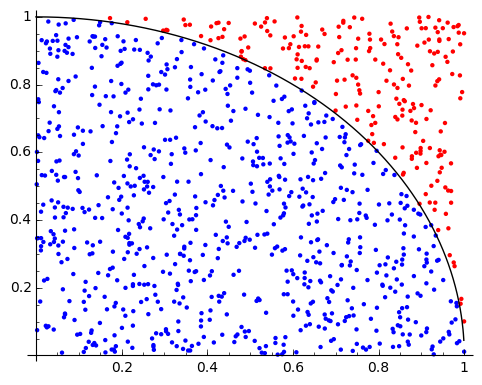
\includegraphics[width=0.5\textwidth]{monte1}
  \end{center}
  \caption{Random sampling in the unit square and circle}
  \vspace{-35pt}
  \vspace{30pt}
\end{wrapfigure}

In this example, we take the unit square constrained by the unit circle (with equation $x^2 + y^2 = 1$). As we take a large amount of random points with the square, we look at the ratio of the number of point in the unit circle over the total number of points in the unit square.

This ratio, call it $\rho$, will come out to be approximately 0.787 $\approx \frac{\pi}{4}$. Since this is only looking at a quarter of the unit circle, we can see how the area is approximated to be $\pi$. \\

On the next page is the source code for the graphic above, using Sage, which includes the code for finding the actual approximation for pi, which is then printed out.


\pagebreak
\noindent \textbf{SAGE code: An approximation of $\pi$}

\noindent\rule{8cm}{0.4pt}
\begin{lstlisting}
#initialize
points_in = []
points_out = []
n = 1000
inside = 0

#place random points
for i in range(0,n):
    [x,y]=[random(),random()]

    if (y <= sqrt(1-(x^2))):
        inside += 1
        points_in.append([x,y])
    else:
        points_out.append([x,y])

# calculate approximation
a = RR(4*(inside / n))
ans = "pi is approximately: %s"%(a)
print ans

#graph solution
circle = []
for i in range(0,1000):
    x = i/1000
    y = sqrt(1-(i/1000)^2)
    circle.append([x,y])

graph = list_plot(points_in, color="blue")
graph += list_plot(points_out, color="red")
graph += list_plot(circle,color="black",figsize=[5,4],plotjoined=true)
show(graph)
\end{lstlisting}
\noindent\rule{8cm}{0.4pt} \\

When the code is run we get that; "pi is approximately: 3.13200000000000" which is obviously very close to the real answer of 3.14, showing that a Monte Carlo approximation is a quite reliable method.

\pagebreak

\subsection{Dice Rolling}

\hspace{4ex} Considering the Monte Carlo methods were developed with a strong connection to statistics and probability as it relates to gambling, a reasonable example would be of the odds of rolling dice. \\

Obviously when rolling two die, the chances of rolling certain numbers are more common than rolling others. Some simple sage code is given on the next page showing a simulation of randomly rolling two die. A figure of the different possibilities for two dice is shown below, including the probability of rolling each respective number.

\begin{center}
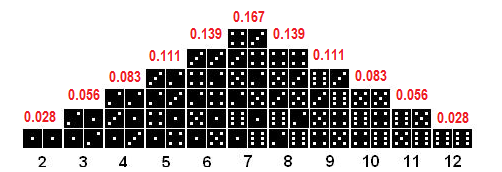
\includegraphics[width=0.75\textwidth]{monte3}
\end{center}

The figure below is one of the random simulations done based on two fair dice being rolled (based on my sage code). After each roll the total of the two dice is recorded, a number between 2 and 12, and the final numbers are plotted.

\begin{center}
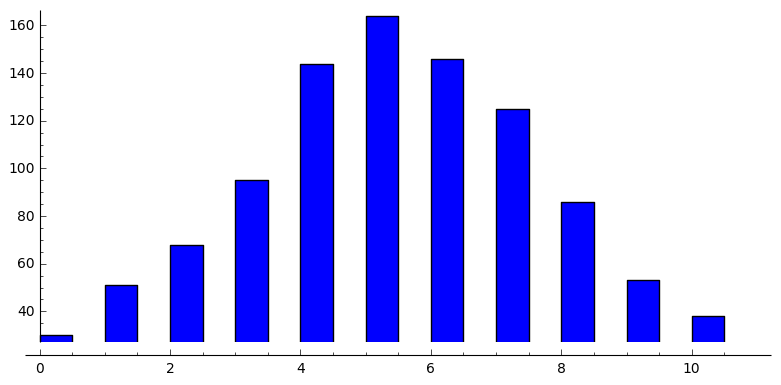
\includegraphics[width=0.75\textwidth]{monte2}
\end{center}

The occurence of each number is then counted and shown in the bar graph. We see that 7 is the most common number rolled, as expected, since there are more ways to roll it.  As you can see the two figures bear a similar resemblance, showing that the Monte Carlo method is suitable in these types of situations.

\pagebreak

\noindent \textbf{SAGE code: Rolling Dice}

\noindent\rule{8cm}{0.4pt}
\begin{lstlisting}
import random
from sage.plot.bar_chart import BarChart

#initialize
dice_throws = []
totals = []
final = []
n = 1000

#roll
for i in range(n):
    [x,y] = [random.randint(1,6),random.randint(1,6)]
    dice_throws.append([x,y])
    totals.append(x+y)
for i in range(2,13):
    final.append(totals.count(i))

#calculate probability
prob = [RR(i/n).n(digits=3) for i in final]; prob

#graph
g = bar_chart(final)
g.show()
\end{lstlisting}
\noindent\rule{8cm}{0.4pt} \\

From one of the random samples used in the code above, the following probabilities of rolling the following values were calculated (also showing actual probabilities):

\begin{table}[h]
\begin{tabular}{l l l l l l l l l}
Total Rolled & 2 & 3 & 4 & 5 & 6 & 7 & 8 \\
Random Sample & 0.0210 & 0.0520 & 0.0830 & 0.127 & 0.148 & 0.159 & 0.156 \\
Actual Probability & 0.028 & 0.056 & 0.083 & 0.111 & 0.139 & 0.167 & 0.139 \\
\end{tabular}
\end{table}

\begin{table}[h]
\begin{tabular}{l l l l l}
Total Rolled & 9 & 10 & 11 & 12 \\
Random Sample &0.0970 & 0.0900 & 0.0470 & 0.0200 \\
Actual Probability &0.111 & 0.083 & 0.056 & 0.028 \\
\end{tabular}
\end{table}

\pagebreak

\section{Real-World Applications}
\subsection{Finance}
\hspace{4ex} One of the most common places Monte Carlo simulation is used in practice is in finance. A clear example of when Monte Carlo simulation is important in the financial world is in credit-risk. The process is similar to the risk analysis by insurance companies I will touch on later, but it is important to show the similarities that are in two different fields.

Banks and other financial institutions set out loans to a debtor. These loans are subject to credit risk, that is risk induced by the fact that some of the debtors may not meet their financial obligations. An example would be not repaying the loan. When this happens, we can say that the debtor defaults, or is in default.

In order to prevent the defaulting debtors from bankrupting the bank, the bank needs some sort of insurance. Therefore, it charges a risk premium for every loan set out, and collects these in an internal bank account called an expected loss reserve, or capital cushion. The question remains, however, how to assess credit risk in order to choose a reasonable risk premium. \\

\textbf{EXAMPLE:}

\begin{quote}
The bank needs to have standards for each loan they give out. These parameters include:

\hspace{4ex}(a) the amount of money subject to be lost

\hspace{4ex}(b) a loss fraction -- the amount lost when the debtor defaults

\hspace{4ex}(c) the probability of the default \\

The 'Loss Variable' is then:

\centerline{L = a * b * Binomial(1, c)}

After initializing this loss variables and take (a) and (b) to be constants, a Monte Carlo simulation can be done to model a loss distribution based on a certain number of runs.
\end{quote}

\subsection{Risk Analysis}
\hspace{4ex} Many insurance companies such as Primera Blue Cross or Liberty mutual deal with risk analysis on a daily basis. When judging risk for outside parties such as pharmaceutical companies, the Monte Carlo approach just might be the best way to analyze the risk of using a new drug before launching it in stores. \\

\textbf{EXAMPLE:}

\begin{quote}
Suppose you have a skin cream being tested. You find that it has an chemical irritant with a mean concentration of 0.02mg (standard deviation = 0.005mg)

You find that the probability of getting irritated by that chemical is between 5/100/mg and 10/100/mg. The risk is then: \\

\centerline{Risk = 0.002mg * 0.075mg = 0.0015}

Based on this, 15 out of every 10,000 users would be irritated by the certain chemical in the cream. Using a Monte Carlo simulation a random set of users would be used, based on the original trial, to test whether or not it is a suitable product for the public.
\end{quote}

In a Monte Carlo simulation, a random value is selected based on the range of estimates. The model is calculated based on this random value. The result of the model is recorded, and the process is repeated. A typical Monte Carlo simulation calculates the model hundreds or thousands of times, each time using different randomly-selected values. This ability to run a model thousands of times showing as good of an approximation as we see is why Monte Carlo methods are extremely important in risk and analysis.

More examples of avoiding risk for hospitals and insurance companies are as follows: \\

\textbf{Avoiding staffing shortages}
\begin{quote}
Simulations can help determine the probability that the appropriate nurse-to-patient ratio will exist during an outbreak or another extreme event. A hospital's level of service can be severely reduced if they are understaffed or lack the ability to help patients in a quick and precise manner. This could incorporate the total number of nurses working in partner hospitals, those involved in direct patient care,  full-time registered nurses and licensed practical nurses. Nurse non-attendence on account of their own family members' wellness can also be analyzed.
\end{quote}

\textbf{Expansion of facilities}
\begin{quote}
For healthcare organizations such as hospitals who are looking to expand, risk analysis technology can offer helpful guidance in developing appropriate budgets and timelines for project completion. Risk analysis forecasts the impact on stakeholders like patients and their families, hospital staff and surrounding business and infrastructure. During the project, risk analysis technology reflects potential deviations from original goal projections. Given the interrelated nature of budgets, schedules and events, it is critical to have a clear view of how they impact one another and the project as a whole.
\end{quote}

\subsection{Natural Disasters}
It is near impossible to guess when natural disasters are going to occur, but it is always a necesity to be as prepared as possible. So if we can't predict when a devastating tornado or hurricane will touch down, or a typhoon will crash onto our shores, how will we be able to stay organized in order to help those in need? \\

\textbf{Hurricane Katrina}

\begin{quote}
In 2005, Hurricane Katrina struck New Orleans. Lousiana promptly created a crisis hotline where people could call to report missing persons. Given the large amount of incoming calls expected, a Monte Carlo simulation was used to approximate the call load they would be getting. This was used to staff the call center appropriately. The schedule was changed according to incoming data such as the time of calls, the average length of phone calls, and deaths. This call center is the reason why a majority of the missing persons found their loved ones during this tragic time.
\end{quote}

\textbf{Guatemala Volcano Evacuation}

\begin{quote}
Volcan de Fuego is an active volcano in Guatemala. Like all active volcanoes, it has the ability to be destructive, being in a populated area. Guatemala’s National Institute for Volcanology created a risk assessment of potential volcanic-related evacuation risks. They took into consideration variables such as time between a possible eruption and a possible hazard hitting a location, along with communication times from authorities and evacuation times. In September 2012, after its largest eruption since 1999, more than 33,000 people within 12 miles of the volcano were evacuated, once again showing the importance of the simulations they ran in advance.
\end{quote}

\pagebreak

\section{Problems with Monte Carlo}

Some issues arise when using Monte Carlo simulation, including but not limited to the following:

\begin{quote}
Typical assumption set used in Monte Carlo simulation assumes normal distributions and correlation coefficients of zero, neither of which are typical in the world of financial markets. \\

It requires more work and does not result in a demonstrably better answer than other techniques. \\

Assumptions are often made in a model to more easily deploy a Monte Carlo simulation. There are very few planners who know how to formally preform operations research, and make these assumptions without know their implications.
\end{quote}

\pagebreak

\begin{thebibliography}
\noindent\bibitem{Heffernan2014}
Heffernan, Randy. "Monte Carlo Simulation and Human Risk." \textit{Risk Management}. N.p., 4 Mar. 2014. Web. 29 May 2014.

\noindent\bibitem{Risk2014}
"Risk and Decision Analysis, Monte Carlo Simulation, Optimization and More." \textit{Palisade}. Palisade Corporation, 2014. Web. 30 May 2014.

\noindent\bibitem{Walters2014}
Walters, Austin G. "Introduction to Monte Carlo Methods." N.p., 30 Apr. 2014. Web. 29 May 2014.
\end{thebibliography}

\end{document}

%sagemathcloud={"zoom_width":125}

